\documentclass[11pt]{article}
\usepackage{tikz}
\usetikzlibrary{tikzmark, calc,backgrounds,arrows,shapes,positioning,fit,svg.path}
\usepackage{pgfplots}
\pgfplotsset{compat=1.15}
\usepackage{ctex}
\usepackage{CJK,CJKnumb}
\usepackage{geometry}
\geometry{left=2cm,right=2cm}%,top=2.5cm,bottom=2.5cm} % 页边距
\geometry{verbose,tmargin=3.8cm,bmargin=3cm,lmargin=3cm,rmargin=3cm} 
\usepackage[breakable]{tcolorbox}
\usepackage{parskip} % Stop auto-indenting (to mimic markdown behaviour)
\usepackage{iftex}
  \ifPDFTeX
    \usepackage[T1]{fontenc}
    \usepackage{mathpazo}
  \else
    \usepackage{fontspec}
    \usepackage[T1]{fontenc}
  \fi
\usepackage{times} % 设置西文字体为Times Roman
\usepackage{xcolor} % Allow colors to be defined
\usepackage{color}
\usepackage{transparent}
\usepackage{graphicx}
\usepackage{import}
% Maintain compatibility with old templates. Remove in nbconvert 6.0
\let\Oldincludegraphics\includegraphics
\usepackage{float}
\floatplacement{figure}{H} % forces figures to be placed at the correct location
\usepackage{enumerate} % Needed for markdown enumerations to work
\usepackage{amsmath} % Equations
\usepackage{amssymb} % Equations
\usepackage{mathtools}
\usepackage{gensymb}
\usepackage{textcomp} % defines textquotesingle
\usepackage{upquote} % Upright quotes for verbatim code
\usepackage{eurosym} % defines \euro
\usepackage[mathletters]{ucs} % Extended unicode (utf-8) support
\usepackage{fancyvrb} % verbatim replacement that allows latex
\usepackage{fancyhdr}
\usepackage{grffile} % extends the file name processing of package graphics 
                    % to support a larger range
\usepackage{pdfpages}
\makeatletter % fix for old versions of grffile with XeLaTeX
\@ifpackagelater{grffile}{2019/11/01}
{
  % Do nothing on new versions
}
{
  \def\Gread@@xetex#1{%
    \IfFileExists{"\Gin@base".bb}%
    {\Gread@eps{\Gin@base.bb}}%
    {\Gread@@xetex@aux#1}%
  }
}
\makeatother
\usepackage[Export]{adjustbox} % Used to constrain images to a maximum size
\adjustboxset{max size={0.9\linewidth}{0.9\paperheight}}
% 超链接颜色配置
\usepackage[colorlinks,linkcolor=blue,anchorcolor=blue,citecolor=blue,urlcolor=blue]{hyperref}
% The default LaTeX title has an obnoxious amount of whitespace. By default,
% titling removes some of it. It also provides customization options.
% \usepackage[clash]{titling}
\usepackage{longtable} % longtable support required by pandoc >1.10
\usepackage{booktabs}  % table support for pandoc > 1.12.2
\usepackage[inline]{enumitem} % IRkernel/repr support (it uses the enumerate* environment)
% \usepackage[normalem]{ulem} % ulem is needed to support strikethroughs (\sout)
                            % normalem makes italics be italics, not underlines
% \usepackage{mathrsfs}
\usepackage{titlesec}

% 设置字体和字号
\setCJKfamilyfont{hwxw}{STXinwei} % 华文新魏
\newcommand{\hwxw}{\CJKfamily{hwxw}}
\newCJKfontfamily{\cusongti}[AutoFakeBold={3.17}]{SimSun} % 伪加粗-宋体
\newcommand{\chuhao}{\fontsize{42pt}{\baselineskip}\selectfont}
\newcommand{\xiaochuhao}{\fontsize{36pt}{\baselineskip}\selectfont}
\newcommand{\yihao}{\fontsize{28pt}{\baselineskip}\selectfont}
\newcommand{\erhao}{\fontsize{21pt}{\baselineskip}\selectfont}
\newcommand{\xiaoerhao}{\fontsize{18pt}{\baselineskip}\selectfont}
\newcommand{\sanhao}{\fontsize{15.75pt}{\baselineskip}\selectfont}
\newcommand{\sihao}{\fontsize{14pt}{\baselineskip}\selectfont}
\newcommand{\xiaosihao}{\fontsize{12pt}{\baselineskip}\selectfont}
\newcommand{\wuhao}{\fontsize{10.5pt}{\baselineskip}\selectfont}
\newcommand{\xiaowuhao}{\fontsize{9pt}{\baselineskip}\selectfont}
\newcommand{\liuhao}{\fontsize{7.875pt}{\baselineskip}\selectfont}
\newcommand{\qihao}{\fontsize{5.25pt}{\baselineskip}\selectfont}

% 重载章节样式
\renewcommand{\thesection}{\chinese{section}} % 节计数器-汉字
\renewcommand{\thesubsection}{\arabic{subsection}} % 子节计数器-数字
\titleformat{\section}{\Large\bfseries\cusongti}{\thesection、}{0em}{} % 节样式
\titleformat{\subsection}{\large\bfseries}{\thesubsection.}{0.5em}{} % 子节样式
\renewcommand{\today}{\number\year\ / \number\month\ / \number\day } % 日期样式

% 自定义页眉和页脚
\pagestyle{fancy}
\fancyhead[L]{} % 页眉左
\fancyhead[C]{哈尔滨工业大学(深圳)\ 可见光通信\ 实验报告} % 页眉中
\fancyhead[R]{} % 页眉右
\fancyfoot[L]{} % 页脚左
\fancyfoot[C]{\thepage} % 页脚中
\fancyfoot[R]{} % 页脚右
\renewcommand{\headrulewidth}{0pt} % 页眉线宽
\renewcommand{\footrulewidth}{0pt} % 页脚线宽
\makeatletter % 双线页眉(重载)
\def\headrule{{\if@fancyplain\let\headrulewidth\plainheadrulewidth\fi %
\hrule\@height 1.5pt \@width\headwidth\vskip1pt % 上面线为1pt粗
\hrule\@height 0.5pt\@width\headwidth  % 下面0.5pt粗
\vskip-2\headrulewidth\vskip-1pt}      % 两条线的距离1pt
  \vspace{6mm}}     % 双线与下面正文之间的垂直间距
\makeatother

% 水印设置(此处用于插入首页logo)
\usepackage[firstpage,pos={0.5\paperwidth,0.2\paperheight},angle=0]{draftwatermark} % 只有第一页加水印
\SetWatermarkText{\scalebox{0.8}{
\includegraphics{Logo_HIT_blue.pdf}}} % 设置水印logo
\SetWatermarkLightness{1} % 设置水印透明度 0-1
\SetWatermarkScale{0.75} % 设置水印大小 0-1  

% 定义重载列表间距命令
\providecommand{\tightlist}{\setlength{\itemsep}{0pt}\setlength{\parskip}{0.2pt}}
% 定义环境:证明
\newenvironment{proof}{{\heiti 证明:}}{\hfill $\square$\par}

% 报告首页-标题
\title{
  \vspace{6cm}\linespread{2}\selectfont
  \scalebox{0.9}[1]{\xiaochuhao{\hwxw 哈尔滨工业大学{\yihao(深圳)}}}\\
  \scalebox{0.9}[1]{\xiaochuhao{\hwxw 可见光通信实验报告}}\\
  \ \\
  \textbf{\cusongti 实验二:单载波调制-归零和非归零码}
  }
\author{
  \newline\\
  \newline\\
  \newline\\
  \linespread{1.75}\selectfont
  \begin{tabular}{rc}
  \makebox[4em][s]{\textbf{姓\hspace{\fill}名}}:& \underline{\makebox[10em][c]{\textbf{张三}}}\\
  \makebox[4em][s]{\textbf{专\hspace{\fill}业}}:& \underline{\makebox[10em][c]{\textbf{通信工程}}}\\
  \makebox[4em][s]{\textbf{学\hspace{\fill}号}}:& \underline{\makebox[10em][c]{000000000}}\\
  \makebox[4em][s]{\textbf{日\hspace{\fill}期}}:& \underline{\makebox[10em][c]{\today}}
  \end{tabular}}
\date{}

% 用于插入MATLAB代码环境(配合mcode.sty使用)
\usepackage{listings}
\usepackage[framed,numbered,autolinebreaks]{mcode} % 带框、行号、自动断行等属性
\AtBeginEnvironment{lstlisting}{\linespread{1}\selectfont}


%% 正文部分
\begin{document}

% 报告首页
\begin{titlepage}
  \maketitle
  \thispagestyle{empty}
\end{titlepage}

% 正文首页-大标题
\begin{center}
{\erhao \textbf{\cusongti 实验一}}  
\end{center}
% \setcounter{section}{0}

\section{实验原理}
普通功率放大器非线性可以用 Solid State Power Amplifier(SSPA)模型来描述: 
\begin{equation}
  v_{out}(v_{in})= \frac{v_{in}}{\left( 1+\left( \dfrac{v_{in}}{v_{\mathrm{max}}} \right)^{2k}  \right)^\frac{1}{2k}}
\end{equation}
其中, $v_{in}$代表放大器输入电压;$v_{out}$是放大器输出电压;$v_{\mathrm{max}}$是最大输出(饱和) 电压;$k$为膝盖因子(knee factor),控制 LED 顶部线性区域到非线性(饱和)区域过渡的平滑程度。

LED 作为可见光通信的发送端,类似功率放大器,也存在明显的非线性特性。
借鉴 SSPA 模型,LED 非线性伏安模式$i_{LED}(v_{LED})$表示如下:
\begin{equation}
  i_{LED}(v_{LED})=
  \begin{dcases}
    h(v_{LED}), \quad & v_{LED}\geq 0\\
    0, & v_{LED}<0
  \end{dcases}
\end{equation}
其中, $v_{LED}$和$i_{LED}$分别表示 LED 的输入电压和驱动电流,
\begin{equation}
  h(v_{LED})= \frac{f(v_{LED})}{\left( 1+\left( \dfrac{f(v_{LED})}{i_{\mathrm{max}}} \right)^{2k}  \right)^\frac{1}{2k}}
\end{equation}
其中, $i_{\mathrm{max}}$表示经过 LED 的最大驱动直流电流,$f(v_{LED})$是 LED 伏安特性函数,表示为:
\begin{equation}
  f(v_{LED})=\frac{v_{LED}}{R}
\end{equation}
其中,电阻 $R=1 ~\Omega$。

\section{仿真实现}
备注:
\begin{enumerate}
  \tightlist
  \item 回答实验指导书的相关问题。
  \item 仿真代码,并附上关键代码分析。
  \item 仿真结果图。
\end{enumerate}
\subsection{问题1}
已知$i_{\mathrm{max}} = 0.5 \mathrm{~A}$,在膝盖因子 $k = 2, 3, 50$ 情况下(在一个仿真图里显示),要求用 MATLAB 模拟仿真出 LED 非线性伏安模型(输入电压$v_{LED}$和经过 LED 电流$i_{LED}$之间的关系)。注意$v_{LED}$取值在-0.5V和 1V 范围内,步长设置为 0.1V。

\subsubsection*{仿真结果}
\begin{figure}
  \centering
  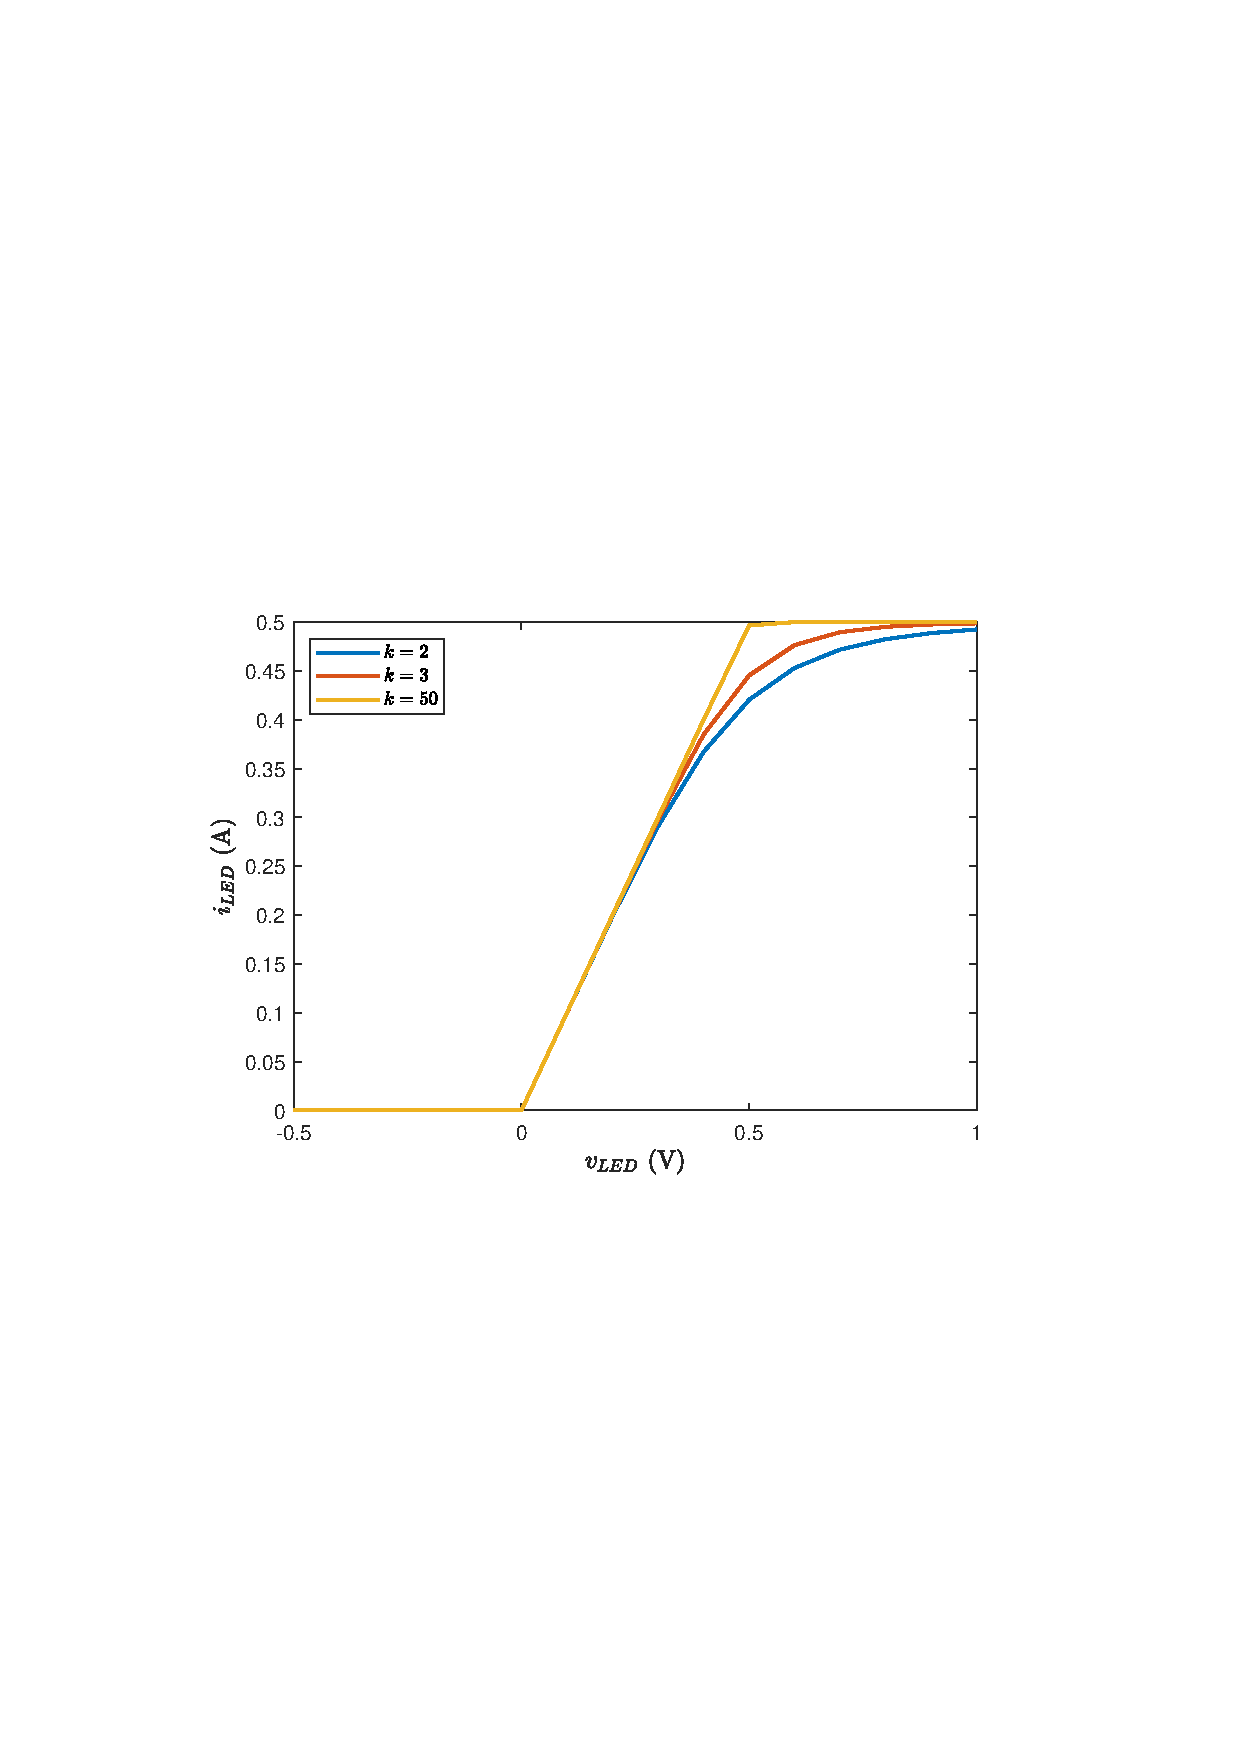
\includegraphics[width=\textwidth]{fig1.pdf}
  \label{fig:1}
\end{figure}

\subsubsection*{程序代码}
\begin{lstlisting}
% Setting Parameters
R = 1;
k = [2 3 50];
v = [-0.5:0.1:1];
vlen = length(v);
imax = 0.5;
% Calculating Results
res = zeros(3, vlen);
for kk = 1:3
    res(kk, :) = get_est(v, imax, k(kk));
end
% Plotting Figures
plot(v, res(1,:), v,res(2,:), v, res(3,:), 'linewidth', 1.5);
legend('$k=2$', '$k=3$', '$k=50$', 'interpreter', 'latex', 'location', 'northwest');
xlabel('$v_{LED}$ (V)', 'interpreter', 'latex', 'fontsize', 12);
ylabel('$i_{LED}$ (A)', 'interpreter', 'latex', 'fontsize', 12);

% Getting i_LED by v_LED vector
function a_est = get_est(vec, imax, k)
    a_est = vec;
    for j = 1:length(vec)
        a_est(j) = h(vec(j), imax, k);
    end
end
% Function f(v)
function g = f(v)
    global R
    g = v./R;
end
% Function h(v)
function i = h(v, imax, k)
    if v >= 0
        g = f(v);
        i = g./((1+(g./imax).^(2.*k)).^(1./(2.*k)));
    else
        i = 0;
    end
end
\end{lstlisting}

\subsection{问题2}
\begin{enumerate}[label = \alph*)]
  \item 根据 OSRAM Golden DRAGON W5AM 的 Data Sheet 数据,回答此型号 LED 的开启电压是多少?
  
  \textbf{答:} 此型号 LED 的开启电压是2.77V。
  \item LED 的非线性模型可以展示 LED 顶部的非线性特性,却不能够体现出LED 底部开启电压之后的非线性特性。一个常用的改进方法是使用拟合的方式得到$f(v_{LED})$。根据 Data Sheet 数据,用 MATLAB 拟合工具找到最佳匹配的公式来表示 LED 非线性模型中的伏安特性函数,代替公式(4),以此得到新的 LED 伏安特性函数。在 MATLAB 上拟合出实际 LED 灯的伏安特性曲线并与 Data Sheet 的数据进行对比,给出拟合出来的 LED 灯的伏安特性函数表达公式,并回答最大驱动直流电流$i_{\mathrm{max}}$和膝盖因子$k$各为多少?
  
  \textbf{答:} 用二次多项式拟合出来的 LED 灯的伏安特性函数表达公式为$$f(x)=1.1985x^{2}+0.2519x+0.0016$$如实验结果图所示,最大驱动直流电流$i_{\mathrm{max}}$和膝盖因子$k$可以有多种取值组合使得与拟合曲线的均方差最小,比较典型的一组为$i_{\mathrm{max}}=2.21 \mathrm{~A},\ k=4.11$。(图中列出了三组,分别为膝盖因子$k$取值最小化、中间取值以及最大驱动直流电流$i_{\mathrm{max}}$取值最小化对应的情况。)
  \item 注意: 
  \begin{itemize}
      \tightlist \small
    \item 拟合的时候推荐二次多项式,并需要把 Data Sheet 中的电压去除开启电压值之后再拟合,最后再加上开启电压值。
    \item 最大驱动直流电流$i_{\mathrm{max}}$和膝盖因子$k$需要重新调整,可以使用最小均方差方法搜索,最大驱动直流电流$i_{\mathrm{max}}$处于0-3A范围之间,步长为0.01A;膝盖因子$k$位于0-5之间,步长为 0.01;电压取值范围为0-5 V 之间,步长为0.01。
  \end{itemize}
\end{enumerate}

\section{仿真结果分析与总结}
备注:
\begin{enumerate}
  \tightlist
  \item 对仿真结果进行分析。
  \item 对本次实验进行总结和思考。
\end{enumerate}
\subsection{对SSPA模型一些结论的推导}
根据公式(1),我们有以下结论
\begin{enumerate}
  \item $0\leq v_{out}(v_{in})< v_{\mathrm{max}}$
  
  \begin{proof}
    要证明以上结论,即要证$\displaystyle 0\leq \frac{x}{\left( 1+x^{k}  \right)^\frac{1}{k}}<1,\quad (x\geq 0)$\\
    \begin{itemize}
        \tightlist
      \item 对于$\displaystyle \frac{x}{\left( 1+x^{k} \right)^\frac{1}{k}}\geq 0$,由$x\geq 0$易得。
    同时,要使$\displaystyle \frac{x}{\left( 1+x^{k} \right)^\frac{1}{k}}= 0$当且仅当$x= 0$。
      \item 对于$\displaystyle \frac{x}{\left( 1+x^{k} \right)^\frac{1}{k}}<1$,即
    \begin{align*}
      &\implies x < \left( 1+x^{k} \right)^\frac{1}{k}\\
      &\implies x^k < 1 +x^{k}
    \end{align*}
      \item 同时有结论 $\displaystyle \lim_{v_{in} \to \infty} v_{out}(v_{in}) = v_{\mathrm{max}}$,即$\displaystyle \lim_{x \to \infty}\frac{x}{\left( 1+x^{k}  \right)^\frac{1}{k}}=1\implies \lim_{x \to \infty}\frac{x^k}{ 1+x^{k}  }=1$
    \end{itemize}
  \end{proof}
  \item $ v_{out}(v_{in})< v_{in} $
  
  \begin{proof}
    要证明以上结论,即要证$\displaystyle \frac{x}{\left( 1+x^{k}  \right)^\frac{1}{k}}<x,\quad (x\geq 0)$
    \begin{align*}
      &\implies \frac{1}{\left( 1+x^{k}  \right)^\frac{1}{k}}<1\\
      &\implies 1 < \left( 1+x^{k}  \right)^\frac{1}{k} \\
      &\implies 1 = 1^k <  1+x^{k}
    \end{align*}
  \end{proof}
\end{enumerate}
由函数图像可以直观看出以上结论的特点。
\definecolor{dpurple}{rgb}{0.39,0.34,0.82}
\definecolor{dblue}{rgb}{0.08,0.39,0.752}
\definecolor{dgreen}{rgb}{0.18,0.49,0.19}
\definecolor{dred}{rgb}{0.82,0.18,0.18}
\definecolor{dorange}{rgb}{0.858,0.38,0.07}
\begin{figure}[htpb]
  \centering
  \begin{tikzpicture}[line cap=round,line join=round,>=triangle 45,x=5cm,y=5cm]
    \begin{axis}[
    ticks=none,
    x=3.5cm,y=3.5cm,
    axis lines=middle,
    xmin=-0.2,
    xmax=3.4,
    ymin=-0.2,
    ymax=1.4,
    xlabel={$x$},
    ylabel={$y$},
    name=border,]
    \draw[line width=1.2pt,color=dred,domain=0.01:2.5] plot (\x, {\x/(exp((1/10)*ln(1+exp(10*ln(\x)))))});
    \draw[line width=1.2pt,color=dorange,domain=0.01:2.5] plot (\x, {\x/(exp((1/3)*ln(1+exp(3*ln(\x)))))});
    \draw[line width=1.2pt,color=dgreen,domain=0.01:2.5] plot (\x, {\x/(exp((1/2)*ln(1+exp(2*ln(\x)))))});
    \draw[line width=1.2pt,color=dblue,domain=0.01:2.5] plot (\x, {\x/(exp((1/1.5)*ln(1+exp(1.5*ln(\x)))))});
    \draw[line width=1.2pt,color=dpurple,domain=0.01:2.5] plot (\x, {\x/(exp((1)*ln(1+exp(ln(\x)))))});
    \draw[dashed, line width=0.7pt] (0,0)--(1,1)--(0,1);
    \draw[dashed, line width=0.7pt] (1,1)--(2.5,1);
    \draw (-0.15,0.15) node[anchor=north west] {$O$};
    \draw[color=gray] (0.52,0.68) node {$y=x$};
    \draw[color=gray] (0.62,1.08) node {$y=x_{\mathrm{max}}$};
    \end{axis}
    \node[draw=black,fill=white,below left=2mm] at (border.north east) {%
    \begin{scriptsize}
    \begin{tabular}{@{}r@{ }l@{}}
     \raisebox{2pt}{\tikz{\draw[line width=1.2pt,color=dred] (0,0) -- (5mm,0);}}&$\dfrac{x}{\left(1+x^{10}  \right)^{\frac{1}{10}}}$\vspace*{0.5em}\\
     \raisebox{2pt}{\tikz{\draw[line width=1.2pt,color=dorange] (0,0) -- (5mm,0);}}&$\dfrac{x}{\left({1+x^{3}}  \right) ^{\frac{1}{3}}}$\vspace*{0.5em}\\
     \raisebox{2pt}{\tikz{\draw[line width=1.2pt,color=dgreen] (0,0) -- (5mm,0);}}&$\dfrac{x}{\left({1+x^{2}}  \right) ^{\frac{1}{2}}}$\vspace*{0.5em}\\
     \raisebox{2pt}{\tikz{\draw[line width=1.2pt,color=dblue] (0,0) -- (5mm,0);}}&$\dfrac{x}{\left({1+x^{1.5}}  \right) ^{\frac{1}{1.5}}}$\vspace*{0.5em}\\
     \raisebox{2pt}{\tikz{\draw[line width=1.2pt,color=dpurple] (0,0) -- (5mm,0);}}&$\frac{x}{{1+x}}$
    \end{tabular}
  \end{scriptsize}};
  \end{tikzpicture}
\end{figure}

\subsection{仿真结果分析}
\subsubsection*{分析:问题1}
\begin{itemize}
    \tightlist
  \item 由仿真结果,可以验证上面对SSPA模型一些结论的推导的正确性。
  \item 在开启电压附近的范围内,曲线斜率大、上升速度快;达到一定的电压值后曲线上升速度减缓,且逐渐趋近于$i_{\mathrm{max}}$值。
  \item 同时,当$k$越小,曲线变化越平滑;当$k$越大,曲线变化速率越快,很快就达到$i_{\mathrm{max}}$值。
\end{itemize}
\subsubsection*{分析:问题2}
\begin{itemize}
  \tightlist
\item 由拟合出的二次曲线是一条开口向上、顶点近似在横轴上的抛物线。
\item 如图(“$\sigma$ changes by $i_{\mathrm{max}}$ and $k$”)所示,与拟合曲线的均方差随着最大驱动直流电流$i_{\mathrm{max}}$和膝盖因子$k$的增加而单调递减,但递减幅度逐渐减小,使得均方差收敛为固定值。
\item 如实验结果图所示,最大驱动直流电流$i_{\mathrm{max}}$和膝盖因子$k$可以有多种不同的取值组合得到满足要求的拟合效果,比较典型的一组为$i_{\mathrm{max}}=2.21 \mathrm{~A},\ k=4.11$。(实验结果图中列出了三组,分别为膝盖因子$k$取值最小化、中间取值以及最大驱动直流电流$i_{\mathrm{max}}$取值最小化对应的情况。)
\end{itemize}

\subsection{实验总结}
本次实验总体难度不大,拟合部分主要在于使用MATLAB中的\mcode{p = polyfit(x,y,n);}语句进行多项式曲线拟合,以及\mcode{y = polyval(p,x);}语句进行多项式计算;寻找最大驱动直流电流$i_{\mathrm{max}}$和膝盖因子$k$则是简单的循环遍历以及用\mcode{S = std(A);}语句计算标准差,以便找到最小均方误差的取值;在实验过程中进一步熟悉了\mcode{function}函数、画图以及其他MATLAB使用方法。
感谢老师和助教的悉心指导。

% 另起一页,添加附录
\newpage
\appendix
% 重新定义页眉页脚规则
\pagestyle{fancy}
\setlength{\topmargin}{-8mm}
\fancyhead[L]{附件:Data Sheet}
\fancyhead[C]{}
\fancyhead[R]{}
\fancyfoot[L]{}
\fancyfoot[C]{}
\fancyfoot[R]{}
\renewcommand{\headrulewidth}{0pt}
\renewcommand{\footrulewidth}{0pt}
\makeatletter % 重载headrule
\def\headrule{}
\makeatother
% 插入PDF
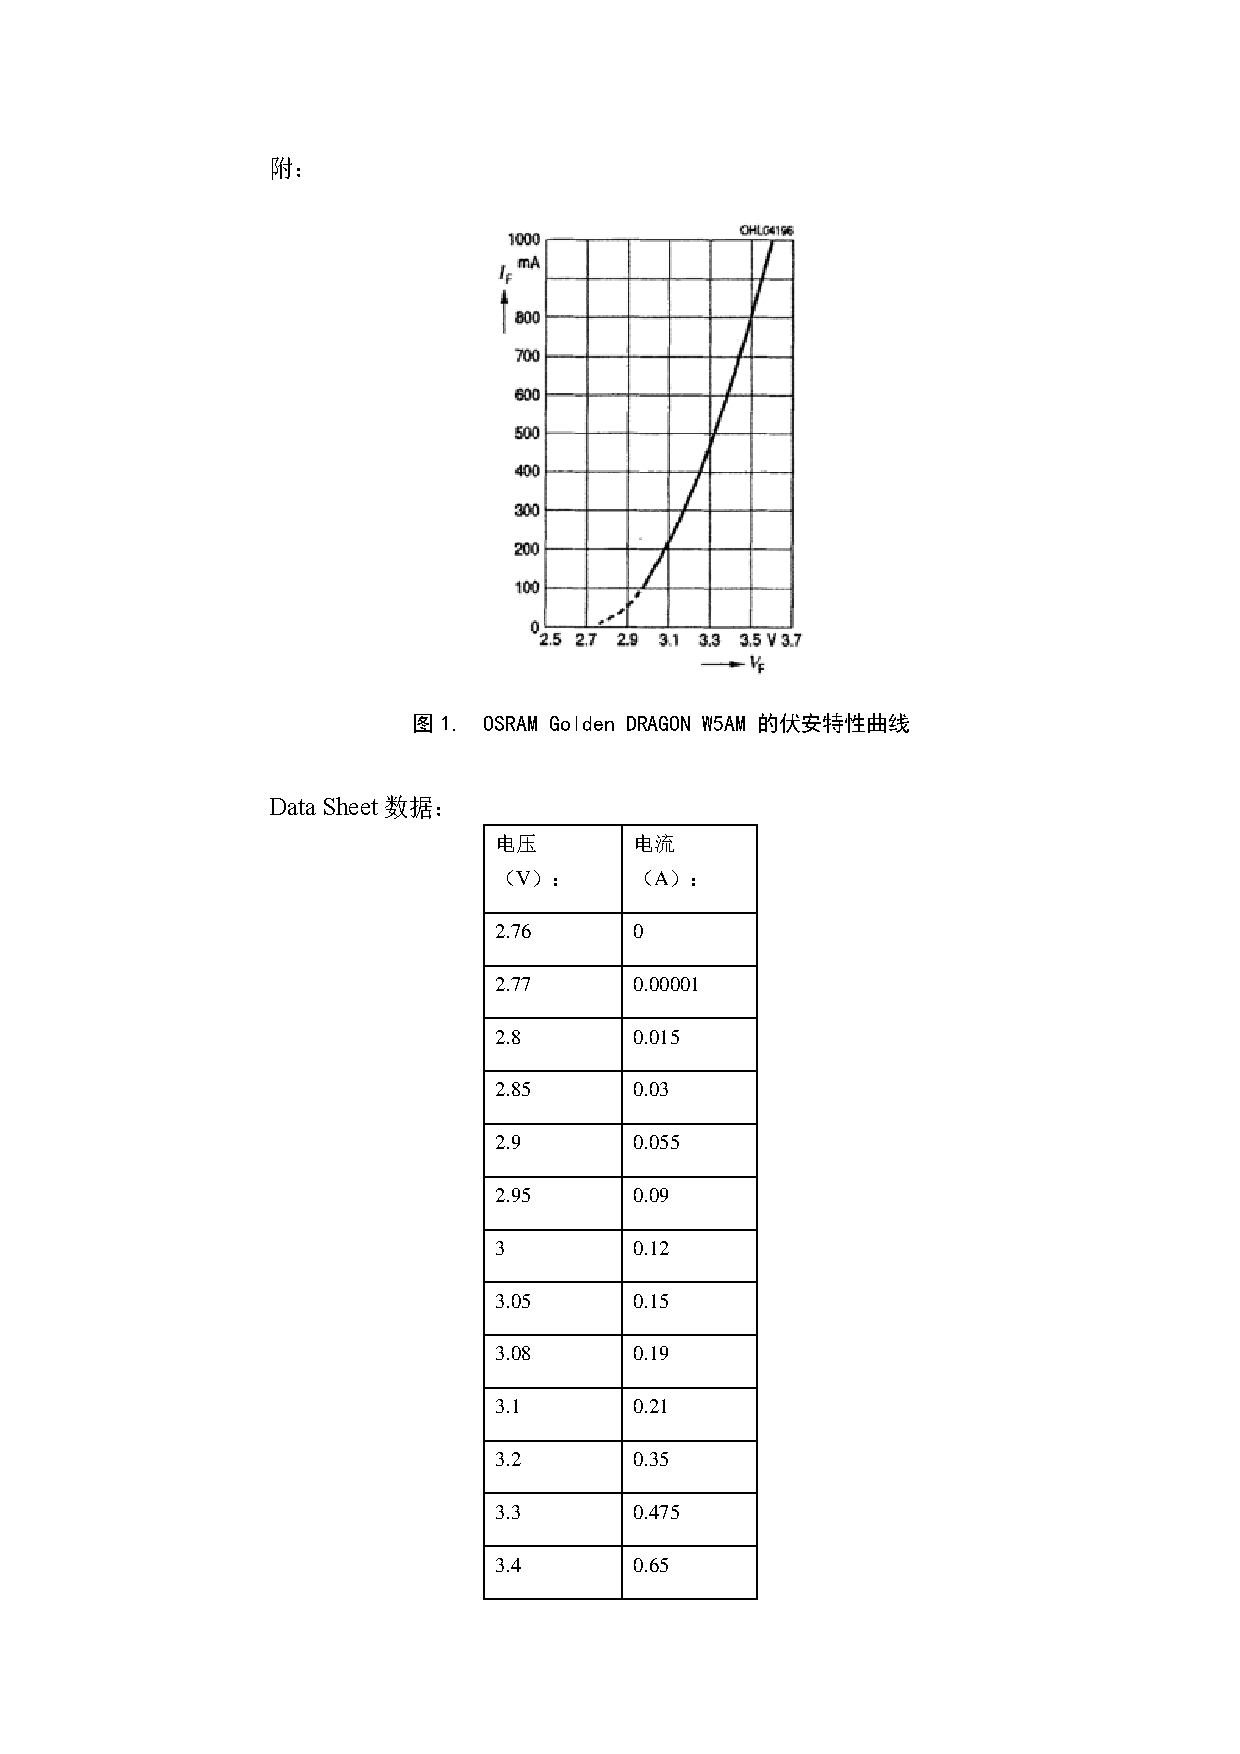
\includepdf[pages=-, pagecommand={\pagestyle{fancy}}]{data_sheet.pdf}

\end{document}